%%%%%%%%%%%%%%%%%%%%%%%%%%%%%%%%%%%%%%%%%%%%%%%%%%%%%%%%%%%%%%%%%%%%%%%%%%%%%
\documentclass[onecolumn, 12pt]{article}

%%%%%%%%%%%%%%%%%%%%%%%%%%%%%%%%%%%%%%%%%%%%%%%%%%%%%%%%%%%%%%%%%%%%%%%%%%%%%
% Used Packages
%%%%%%%%%%%%%%%%%%%%%%%%%%%%%%%%%%%%%%%%%%%%%%%%%%%%%%%%%%%%%%%%%%%%%%%%%%%%%
\usepackage[T1]{fontenc}
\usepackage{times}
\usepackage{amsfonts}
\usepackage{amsmath}
\usepackage{graphicx}
\usepackage{color}
\usepackage{multicol}
\usepackage{amssymb}
\usepackage{subfigure}
\usepackage{bm}
\usepackage{latexsym}
\usepackage{stfloats}
\usepackage{mathtools}
\usepackage{caption}
\usepackage[unicode,colorlinks, linkcolor=black,anchorcolor=black,citecolor=black]{hyperref}
\usepackage[toc, page]{appendix}

\usepackage{caption}
\captionsetup[lstlisting]{font={small,tt}}

%\usepackage{geometry}
%\geometry{letterpaper, total={216mm,279mm}, left=25mm, right=25mm, top=20mm, bottom=20mm}

\setlength{\hoffset}{-0.5in}
\setlength{\voffset}{-0.6in}
\addtolength{\textwidth}{1.1in}
\addtolength{\textheight}{1in}


\usepackage{listings}
% NOTE: THIS IS THE WRONG WAY TO DO THIS!!!  FIX IT!
\usepackage{courier}  % set bold typewrite font for keyword in c++
\lstset{
language = C++,
basicstyle={\small\tt},
%keywordstyle = \color{black}\bfseries,
showspaces=false,
showtabs=false,
showstringspaces=false,
escapechar=@,
escapebegin=\rm,
xleftmargin=4ex,
xrightmargin=0ex,
breaklines=true,
tabsize=4
}

\usepackage{algorithm}
\usepackage{algorithmic}


\begin{document}

\title{Software Description for the M.Eng Project}
\author{
Yue~Tang, V00796163, yuetang@uvic.ca\\
Department of Electrical and Computer Engineering, \\
University of Victoria, Canada.
}
\maketitle



%%%%%%%%%%%%%%%%%%%%%%%%%%%%%%%%%%%%%%%%%%%%%%%%%%%%%%%%%%%%%%%%%%%%%%%%%%
%           Introduction
%%%%%%%%%%%%%%%%%%%%%%%%%%%%%%%%%%%%%%%%%%%%%%%%%%%%%%%%%%%%%%%%%%%%%%%%%%%
{\centering
\section*{TITLE OF PROJECT}
\begin{center}
Complete 3D Triangle Mesh Coding Using Edgebreaker and Parallelogram Prediction
\end{center}}
\newpage


%%%%%%%%%%%%%%%%%%%%%%%%%%%%%%%%%%%%%%%%%%%%%%%%%%%%%%%%%%%%%%%%%%%%%%%%%%
%          TASK DESCRIPTION
%%%%%%%%%%%%%%%%%%%%%%%%%%%%%%%%%%%%%%%%%%%%%%%%%%%%%%%%%%%%%%%%%%%%%%%%%%
\section{TASK DESCRIPTION}
A triangle mesh can be represented by its geometry and by its connectivity. Parallelogram prediction is a simple scheme developed by Touma and Gotsman \cite{Parallel} to compress the vertex coordinates, sometimes called geometry of three-dimensional triangle meshes. The accuracy and simplicity of parallelogram prediction make it very suitable for coding the geometry information of the 3D triangle mesh.

The triangle-vertex incidence table, which associates each triangle's three bounding vertices with triangle's references, is a very good representation of a triangle mesh's connectivity. Edgebreaker is a simple scheme developed by Rossignac \cite{Edgebreaker} to compress the triangle vertex incidence graphs, sometimes called connectivity or topology of 3D triangle meshes. The superior compression capabilities and versatility make Edgebreaker algorithm very suitable for the 3D graphic application.

In this Master of Engineering project, I will implement the complete three-dimensional triangle mesh coding method using the Edgebreaker algorithm and the parallelogram prediction scheme. The Edgebreaker algorithm is used for the connectivity coding, and the parallelogram prediction scheme is used for the geometry coding. Two executable programs are contained in this project, the \lstinline!compression! program and \lstinline!decompression! program, for 3D triangle mesh compression and decompression, respectively.



%%%%%%%%%%%%%%%%%%%%%%%%%%%%%%%%%%%%%%%%%%%%%%%%%%%%%%%%%%%%%%%%%%%%%%%%%%%
%           ALGORITHM
%%%%%%%%%%%%%%%%%%%%%%%%%%%%%%%%%%%%%%%%%%%%%%%%%%%%%%%%%%%%%%%%%%%%%%%%%%%
\section{ALGORITHM} \label{sec:algorithm}
\subsection{Edgebreaker Algorithm}
The Edgebreaker algorithm is independent of the vertex location, and only takes the triangle mesh's connectivity into consideration. For any mesh with $t$ triangles that is homeomorphic to a sphere, the Edgebreaker can encode its connectivity into $2t$ bits or less \cite{Edgebreaker}. Both Edgebreaker's compression and decompression algorithm requires the traversal from one triangle to an adjacent one in the mesh. The topological relation between the current triangle and the boundary of remaining part of the mesh can be described by an op-code produced at each stage of the compression procedure. In Edgebreaker's decompression procedure, the entire connectivity of the original mesh is reconstructed by the op-codes generated during the compression procedure.

\subsubsection{Edgebreaker Compression Algorithm}
Edgebreaker uses five symbols C, L, E, R, and S to identify each triangle's topological relation and appends the selected op-code at the end of the compression history (also called op-code sequence). For triangle mesh with holes, the 5 cases introduced above are not enough to encode this circumstance. Rossignac has proposed a new case, case M, to identify the triangle with its third vertex located at the boundary of the hole. Edgebreaker compression algorithm merges the bounding loop with the hole by opening both loops at their common vertex and reconnecting them into a single cyclic list \cite{Edgebreaker}. Since most of the triangle mesh contains no hole or only one hole, in order to keep the consistency with the simple mesh, and do not introduce new label into the compression history, this M relation can be achieved by modify the already exist S type in the op-code sequence.

Three most important steps involved in the Edgebreaker's compression algorithm are: distinguishing the current triangle topological relation, appending the selected op-code to the compression history, and traversing to the next designated triangle based on the current triangle's op-code.

\subsubsection{Edgebreaker Decompression Algorithm}
The Edgebreaker's decompression algorithm receives a op-code sequence and produces a triangle-vertex incidence table, where each triangle is represented by three labels.

Two traversals of the op-code sequence are required by the Edgebreaker's decompression algorithm. In the first traversal, the decompression preprocessing phase, Edgebreaker decompression algorithm computes the number of triangles, number of exterior vertices, and the offsets for all S operations. In the second traversal, the decompression generation phase, the algorithm creates triangles in the order in which they were deleted by the compression algorithm and assigns the three vertices' label to the triangle.


\subsection{Parallelogram Prediction Scheme}
The parallelogram prediction scheme is used to compress the 3D triangle mesh's geometry information. The scheme encodes the mesh vertex coordinates by first quantizing the three vertex coordinates, then uses the parallelogram prediction scheme to predict the integer coordinates of the vertex. The integer prediction errors are encoded using arithmetic coding scheme and output to the file.

\subsubsection{Vertex Quantization}
Both the compression and decompression program perform the uniformly quantization on each vertex coordinate. The quantization index $k$ we obtained is used in parallelogram prediction scheme. The quantization equation used in the project is:
\begin{align}\label{eq:qunatize}
k =  (sgnx) \left\lfloor{{\frac{\left|x\right|}{\delta}} + {\frac{1}{2}}}\right\rfloor,  \delta \geqslant 0
\end{align}

where $k$ denotes quantization index, $x$ represents the real input coordinate and $\delta$ denotes the quantization step size. The quantization step size can be either entered by user through the command line argument, or calculated based on the input triangle mesh.

The reconstruction rule for this quantizer is simply:
\begin{align}\label{eq:reconstruct}
y = k\cdot \delta
\end{align}


\subsubsection{Parallelogram Prediction}
The rule is called ``parallelogram'' rule since its geometric interpretation is to predict as the fourth vertex of a parallelogram from the other three vertices \cite{Parallel}. It is a simple linear prediction scheme to predict the vertex location from the surrounding vertices on the mesh surface. For third vertex $r$ of triangle incident upon the half edge $g$ (where $u, v$ are the end and beginning vertices bounding the half edge $g$), it already have a previously precessed triangle incident upon $g$ with label $u, v$, and $w$. This enables us to predict the new vertex $r^p$ by using the rule
\begin{align}\label{eq:parallelRule}
r^p = v + u - w
\end{align}

In order to combine parallelogram prediction scheme with Edgebreaker algorithm, Rossignac has proposed 6 different cases \cite{predictScheme} based on the the original parallelogram prediction scheme. All the proposed cases are listed below:

\begin{itemize}
\item Case1, no vertex is known, the predict vertex $r^p$ is defined by
\begin{align}\label{eq:case1}
r^p = \{0, 0, 0\}
\end{align}

\item Case2, one vertex $u$ from the same triangle as $r$ is known, $r^p$ is defined by
\begin{align}\label{eq:case2}
r^p = u
\end{align}

\item Case3, one vertex $v$ from the same triangle as $r$ is known, $r^p$ can be predicted as
\begin{align}\label{eq:case3}
r^p = v
\end{align}

\item Case4, two vertices $u$ and $v$ from the same triangle as $r$ are known, $r^p$ is defined by
\begin{align}\label{eq:case4}
r^p = (u + v) / 2
\end{align}

\item Case5, vertex $u$, and the vertex $w$ from the neighboring triangle are known, $r^p$ can be predicted as
\begin{align}\label{eq:case5}
r^p = 2u - w
\end{align}

\item Case6, all three vertices $u$, $v$ and $w$ are known, the predict vertex $r^p$ is defined by
\begin{align}\label{eq:case6}
r^p = u + v - w
\end{align}
\end{itemize}

The diagram for parallelogram prediction scheme and the six cases can be found in Figure~\ref{fig:parallel}.
\begin{figure}[h]
\centering
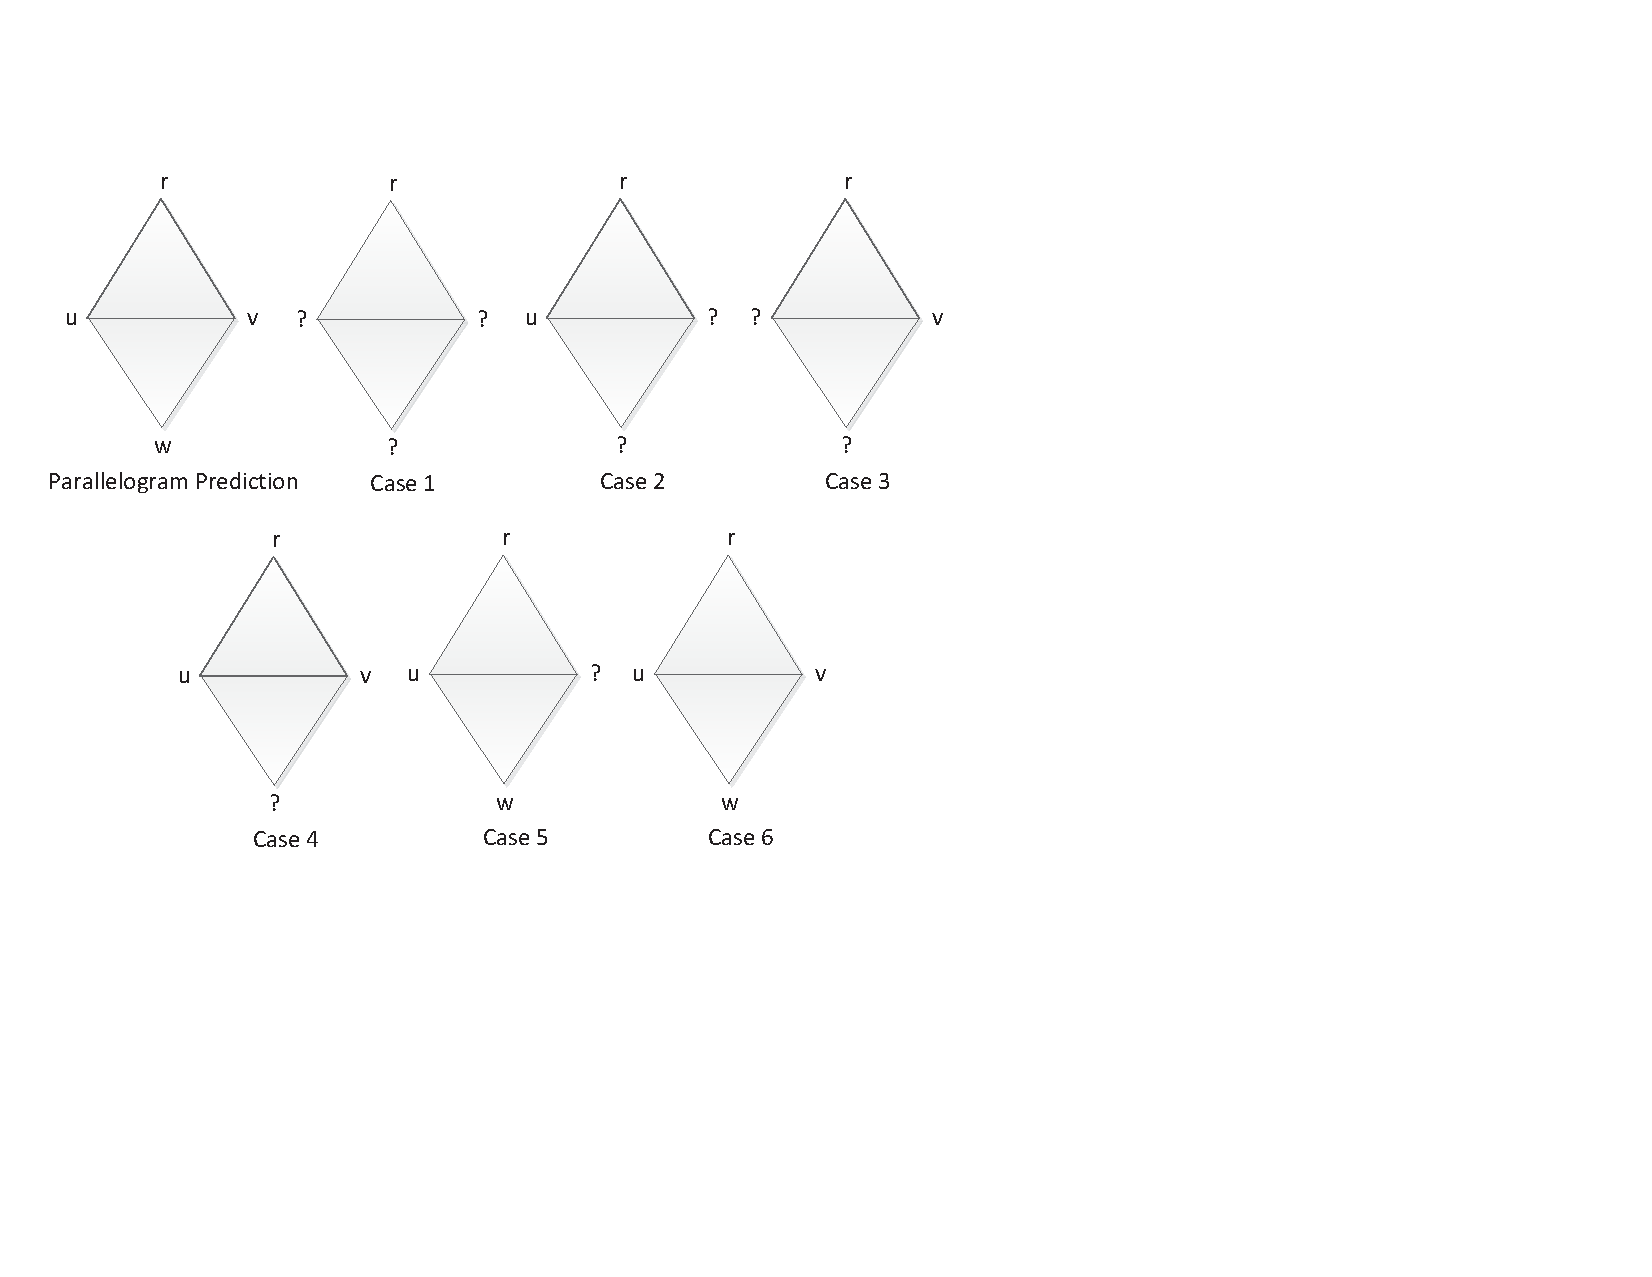
\includegraphics[width=0.6\textwidth, clip, keepaspectratio]{fig_parallel.eps}
\caption{Parallelogram prediction scheme and six cases}\label{fig:parallel}
\end{figure}

The integer prediction errors can be written as:
\begin{align}\label{eq:delta}
\Delta_i = r_i - r^p_i
\end{align}

where $r_i$ denotes the actual vertex coordinate, $r^p_i$ denotes the predicted vertex coordinate, and $\Delta_i$ denotes the integer prediction errors.



%%%%%%%%%%%%%%%%%%%%%%%%%%%%%%%%%%%%%%%%%%%%%%%%%%%%%%%%%%%%%%%%%%%%%%%%%%%
%           SOFTWARE REQUIREMENTS SPECIFICATION
%%%%%%%%%%%%%%%%%%%%%%%%%%%%%%%%%%%%%%%%%%%%%%%%%%%%%%%%%%%%%%%%%%%%%%%%%%%
\section{SOFTWARE REQUIREMENTS SPECIFICATION} \label{sec:SRS}
\subsection{Functionality}
Two executable programs, \lstinline!compression! and \lstinline!decompression!, are contained in the software package for three-dimensional triangle mesh coding. The \lstinline!compression! program reads the triangle mesh in OFF format from the standard input, compresses the triangle mesh and outputs the compressed mesh in the EB file format (to be discussed later). The \lstinline!decompression! program reads the compressed mesh from the standard input, generates the decompressed triangle mesh and writes to standard output in the OFF file format.


\subsection{Build the Software}
The source code for both \lstinline{compression} and \lstinline{decompression} programs are written in C++ language under Linux platform, and should be able to work without any modification to source code on any target machine with a C++ compiler compliant with C++14 standard. The compiler has been used during the software implementation is GCC $5\ldotp 1\ldotp0$.

Besides the C++ standard library, the Computational Geometry Algorithms Library (CGAL) and the Signal/Geometry Processing Library (SPL) are also required. The user needs to guarantee the CGAL and SPL library are successfully installed and executed on the target machine. The library version that has been verified to work with both compression and decompression software is:
\begin{itemize}\itemsep=2pt
\item CGAL: $4\ldotp 2\ldotp 1$
\item SPL: $1\ldotp 1\ldotp 18$
\end{itemize}

The 3D triangle mesh coding software package includes: the source code files for both the compression and decompression program, a Makefile, a sample uncompressed triangle mesh file in OFF format, a sample compressed mesh file in EB format and also a README file.

The \emph{Make} utility is chosen to both compile the source code file and link the object file. To build the compression and decompression software, user needs to change directory into the software package folder, then run the command:
\begin{lstlisting}
make clean
\end{lstlisting}

This \lstinline{make clean} command deletes all the object files and executable files generated from the previous building process and only keep the source code file. To generates all the targets (in our case, both the compression and decompression executable), run the command:
\begin{lstlisting}
make all
\end{lstlisting}


\subsection{External Interface}
As introduced earlier, the software package contains two executable programs: \lstinline{compression} and \lstinline{decompression}.

\subsubsection{Compression Program}
\textbf{Synopsis}
\begin{lstlisting}
compression [OPTION]
\end{lstlisting}


{\setlength\parindent{0pt}
\textbf{Description}\vspace{0.5em}}

This program reads a triangle mesh in OFF file format from standard input, generates the compressed triangle mesh and writes the compressed triangle mesh in EB file format to the standard output. With the command-line options, the user can choose different quantizer step sizes for x, y, and z coordinates. The program returns zero for a normal exit, a nonzero value otherwise.\\


{\setlength\parindent{0pt}
\textbf{Options}\vspace{0.5em}}

\begin{tabular}{l l p{0.75\textwidth}}
\lstinline !-x! & \lstinline !$x_size! & Sets the x coordinate quantization step size to \lstinline !$x_size!. The default value of \lstinline !$x_size! is \lstinline !(x_max - x_min) / 2^16!. The \lstinline !x_max! and \lstinline !x_min! are maximum and minimum x coordinate obtained from the input triangle mesh. \\
\lstinline !-y! & \lstinline !$y_size! & Sets the y coordinate quantization step size to \lstinline !$y_size!. The default value of \lstinline !$y_size! is \lstinline !(y_max - y_min) / 2^16!. The \lstinline !y_max! and \lstinline !y_min! are maximum and minimum y coordinate obtained from the input triangle mesh. \\
\lstinline !-z! & \lstinline !$z_size! & Sets the z coordinate quantization step size to \lstinline !$z_size!. The default value of \lstinline !$z_size! is \lstinline !(z_max - z_min) / 2^16!. The \lstinline !z_max! and \lstinline !z_min! are maximum and minimum z coordinate obtained from the input triangle mesh. \\
\lstinline !-b! & \lstinline !$no_bits! & Sets the number of bits used to compress the vertex coordinate to \lstinline !$no_bits!. The default value of \lstinline !$no_bits! is 16 bits.  \\
\end{tabular}
\label{tab:compressCLI}



\subsubsection{Decompression Program}
\textbf{Synopsis}
\begin{lstlisting}
decompression
\end{lstlisting}


{\setlength\parindent{0pt}
\textbf{Description}\vspace{0.5em}}

This program reads a compressed triangle mesh in EB file format from standard input, generates a decompressed triangle mesh and writes the decompressed mesh in OFF file format to the standard output. The program returns zero for a normal exit, a nonzero value otherwise.\\


{\setlength\parindent{0pt}
\textbf{Options}\vspace{0.5em}}

This program has no options.




%%%%%%%%%%%%%%%%%%%%%%%%%%%%%%%%%%%%%%%%%%%%%%%%%%%%%%%%%%%%%%%%%%%%%%%%%%%
%           FILE FORMAT
%%%%%%%%%%%%%%%%%%%%%%%%%%%%%%%%%%%%%%%%%%%%%%%%%%%%%%%%%%%%%%%%%%%%%%%%%%%
\section{EB FILE FORMAT} \label{sec:EB}
The EB format is a new file format for storing both the connectivity and geometry information of the compressed triangle mesh, the file extension is ``.eb''. EB format is a simple file format. In the EB file, it first stores the connectivity information then followed by the geometry information.

Five main parts are included in the EB file format. The first part is the header part, it gives a brief introduce to content inside the file. The second part related to the binary history string, which is the connectivity information of the mesh. The third part is the M table, this part only occurs if the input triangle mesh contains hole. The fourth part is the M' table, this part is related to mesh's handle. The fifth part is geometry information part. All information contained in EB file are byte aligned. A detailed explanation of each part of the EB file is also included in Table~\ref{tab:EBformat}.

\begin{table}[h]
\normalsize
\centering
\caption{EB file format}
  \begin{tabular}{| l | p{0.7\textwidth} | }
    \hline
    Section & Description \\
    \hline
    Header part & Contains triangle mesh's basic information. Header part includes file signature, binary history string size information, number of holes and handles in mesh, and quantization step size.\\
    \hline
    History part & Contains the mesh's connectivity information. Three different code series are used to generate the final binary history string.\\
    \hline
    M table part & Contains hole's information. M table part only occurs if the input triangle mesh contains hole. \\
    \hline
    M' table part & Contains handle's information. M' table part only occurs if the triangle mesh contains handle. \\
    \hline
    Geometry part &  Contains the mesh's geometry information. Parallelogram prediction scheme is used to generate the geometry prediction for each vertex.\\
    \hline
    \hline
  \end{tabular}
  \label{tab:EBformat}
\end{table}

From the description in Table~\ref{tab:EBformat}, an example EB file diagram is given in Figure~\ref{fig:ebfile}.
\begin{figure}[h]
\centering
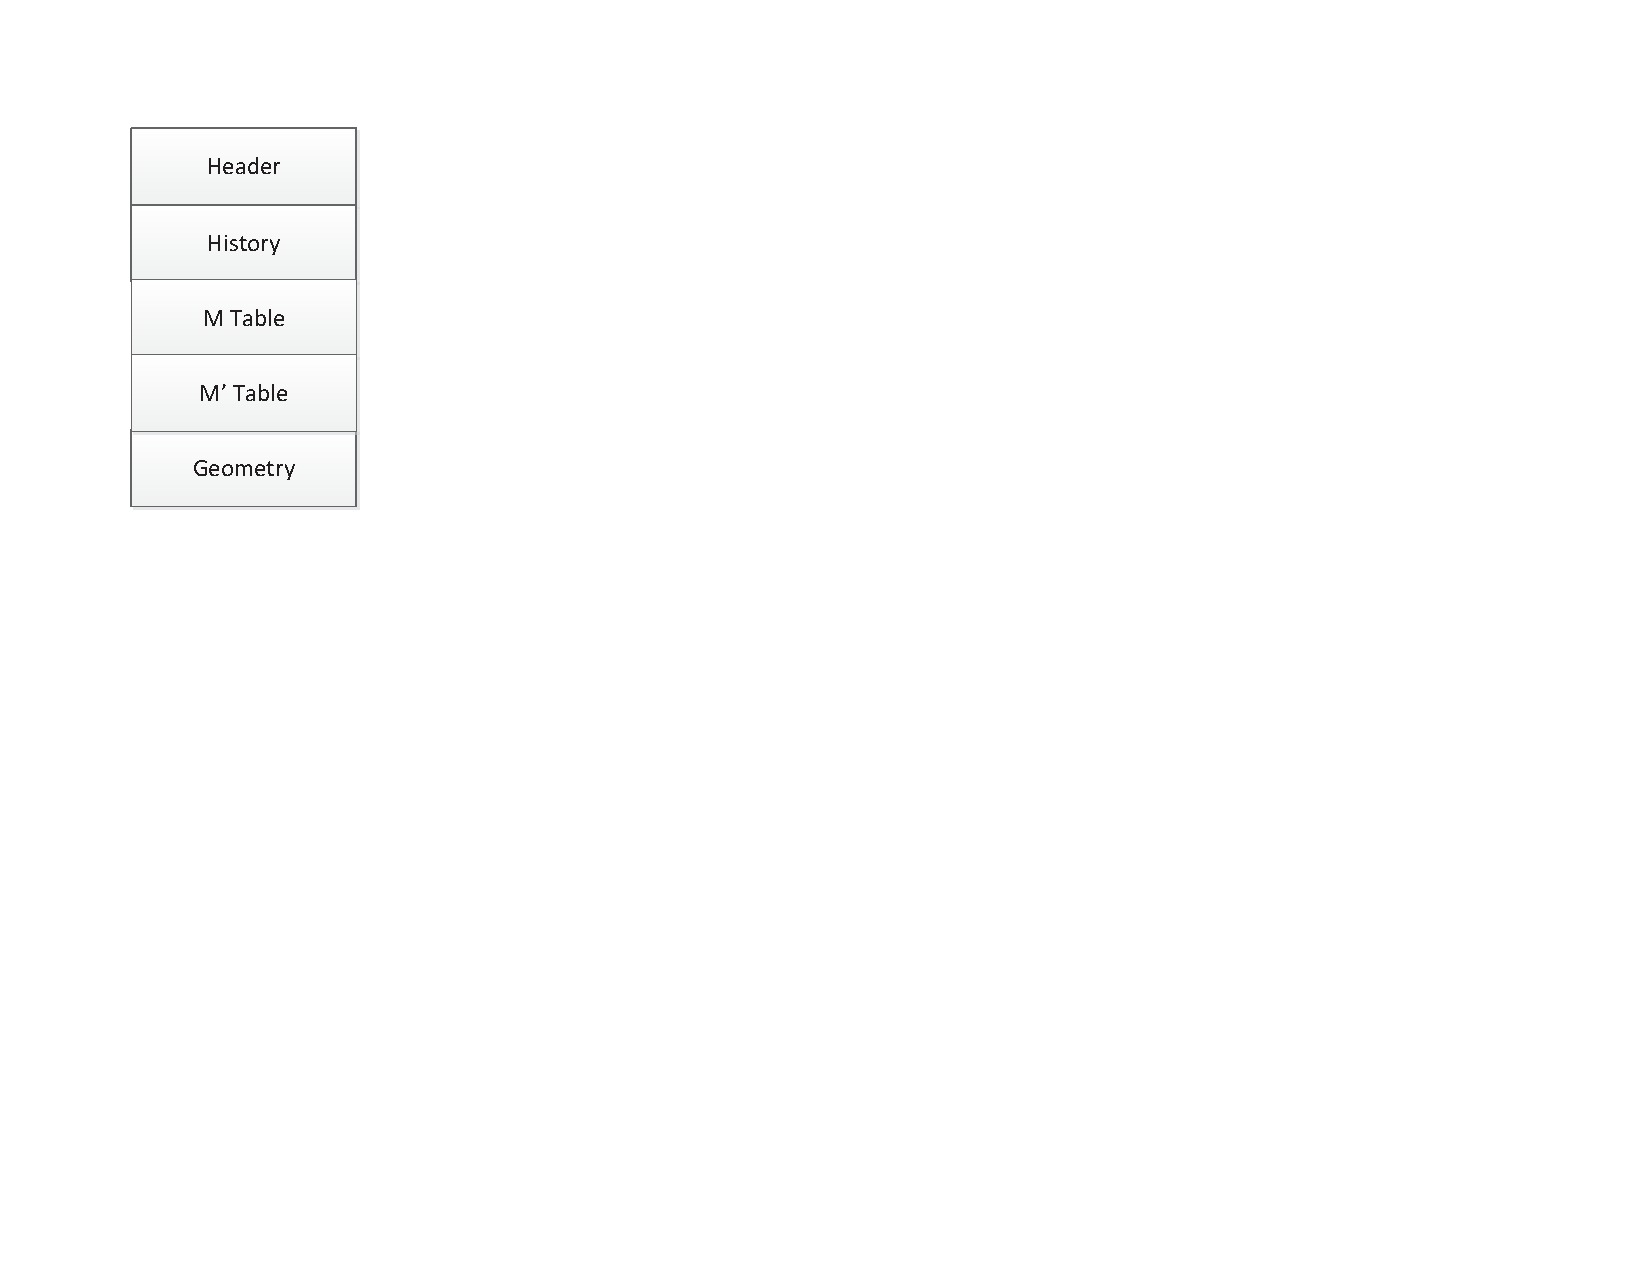
\includegraphics[scale=0.6, clip, keepaspectratio]{fig_ebfile.eps}
\caption{Figure for the example EB file}\label{fig:ebfile}
\end{figure}


\subsection{Header Part}
Several different elements are included in the header part of the EB file. The detailed description are listed below:

\begin{itemize}\itemsep=2pt
\item \lstinline !sig!, 32 bit unsigned integer. Represents the signature of the EB file. The value we choose for file signature is \lstinline!sig! = 696610198.
\item \lstinline !code!, 32 bit unsigned integer. Represents the code series used in the current EB file. Three different binary code series are adopted by both the compression and decompression program.
\item \lstinline !hist_size!, 32 bit unsigned integer. It tracks the number of bytes used to store the binary history strings.
\item \lstinline !hole_count!, 32 bit unsigned integer. Represents number of holes in the mesh.
\item \lstinline !handle_count!, 32 bit unsigned integer. Represents number of handles in the mesh.
\item \lstinline !quan_x quan_y quan_z!, 32 bit unsigned fixed point number with 16 bits for the whole number part and 16 bits for the fractional part. Represents quantization step size for x, y and z coordinate.
\end{itemize}


\subsection{History Part}
The history part contains the connectivity information of the compressed triangle mesh. Based on the work of King and Rossignac \cite{3.67v}, three different binary code series are used for the Edgebreaker algorithm. Three code series used in both compression and decompression program are listed in Table~\ref{tab:codeSeries}. For each code series, a $C$ op-code will be denoted $C_A$ when it immediately follows another $C$ op-code, and $C_N$ otherwise. The similar notation is used for S and R op-codes.

\begin{table}[h]
\normalsize
\centering
\caption{Three binary code series}
  \begin{tabular}{ | p{0.1\textwidth} | p{0.1\textwidth} | p{0.1\textwidth} | p{0.1\textwidth} | }
    \hline
    Opcode & Code 1 & Code 2 & Code 3 \\
    \hline
    $C_A$ & 0 & 0 & 0 \\
    \hline
    $S_A$ & 10 & 10 & 10 \\
    \hline
    $R_A$ & 11 & 11 & 11 \\
    \hline
    \hline
    $C_N$ & 0 & 00 & 00 \\
    \hline
    $S_N$ & 100 & 111 & 010 \\
    \hline
    $R_N$ & 101 & 10 & 011 \\
    \hline
    $L$ & 110 & 110 & 10 \\
    \hline
    $E$ & 111 & 01 & 11 \\
    \hline
    \hline
  \end{tabular}
  \label{tab:codeSeries}
\end{table}

One of the three code series will be chose to generate the final binary history string from the given op-code sequence. After the binary history string is successfully generated, this string will be written to the output EB file.



\subsection{M table Part}
If EB file contains the M table part means the current mesh contains more than one bounding loop and it has M type triangle. The number of holes contained in current triangle mesh can be found in the header part. If \lstinline !hole_count = 0! in the header part, it represents the current triangle mesh doesn't contain any hole.

Two items are included for each hole, the first item is the number of S operation skipped (since in op-code sequence we use S symbol to represent the actual M type triangle, we need a counter to distinguish between the real S and M symbol), and the second item is the length of the hole.

\begin{itemize}\itemsep=2pt
\item \lstinline !skip_count!, 32 bit unsigned integer. Represents number of S operation skipped since the previous M type triangle or since the beginning of the op-code sequence for the first M operation.
\item \lstinline !len!, 32 bit unsigned integer. Represents number of vertices located on current hole's boundary.
\end{itemize}


\subsection{M' table Part}
The M' table part occurs if and only if the triangle mesh contains handle. The number of handles contained in current triangle mesh can be found in the header part. If \lstinline !handle_count = 0! in the header part, it represents the current triangle mesh doesn't contain any handle.

For each handle, 3 items are included in the M' table. The position of the associated gate in the stack, the offset between the gate and the reached point, and the number of S operations skipped after the previous M' operation (we also use the S symbol to represent the actual M' operation in the op-code sequence).

\begin{itemize}\itemsep=2pt
\item \lstinline !position!, 32 bit unsigned integer. Represents the position of the associated gate in the stack.
\item \lstinline !offset!, 32 bit unsigned integer. Represents the offset between the gate and the reached point.
\item \lstinline !skip_count!, 32 bit unsigned integer. Represents number of S operation skipped since the previous M' type triangle or since the beginning of the op-code sequence for the first M' operation.
\end{itemize}


\subsection{Geometry Part}
All the vertices information in the original triangle mesh are stored in the geometry part of the EB file. Parallelogram prediction scheme is used to predict the vertices' position. The integer prediction error between the actual position and predicted position is included in the geometry part. The binary arithmetic coding scheme is used to generate the geometry part of the EB file.



%%%%%%%%%%%%%%%%%%%%%%%%%%%%%%%%%%%%%%%%%%%%%%%%%%%%%%%%%%%%%%%%%%%%%%%%%%%
%           KEY PROCEDURES
%%%%%%%%%%%%%%%%%%%%%%%%%%%%%%%%%%%%%%%%%%%%%%%%%%%%%%%%%%%%%%%%%%%%%%%%%%%
\section{KEY PROCEDURES}
\subsection{Compression Program}
The half edge data structure is used in the compression program. The key procedures contained in the compression program are: mesh preprocessing and triangle mesh compression.


\subsubsection{Data Structure}
The compression program uses the half edge data structure. The \lstinline!CGAL::Polyhedron_3! class from CGAL library is heavily used in the compression program.\\

{\setlength\parindent{0pt}
\textbf{Vertex}\vspace{0.5em}}

According to the Edgebreaker algorithm, three different vertex marks are introduced to the compression program. For the geometry processing, compression program requires each vertex has a unique index number and a boolean type flag to indicate whether the current vertex is processed or not. In order to add mark, index and flag to each vertex, a user defined vertex class named \lstinline!My_Vertex! is used in the compression program. This \lstinline!My_Vertex! class is inherit from the CGAL \lstinline!CGAL::HalfedgeDS_vertex_base! class and some modifications are made based on the program requirements. \\

{\setlength\parindent{0pt}
\textbf{Halfedge}\vspace{0.5em}}

Halfedge marks are also introduced by the Edgebreaker algorithm. During the compression, the program needs to find each border halfedge's predecessor and successor on the current bounding loop. In order to make those changes, a user defined halfedge class is adopted by the compression program. This user defined halfedge class is inherit from the CGAL \lstinline!CGAL::HalfedgeDS_halfedge_base! class, and some modifications are made based on the program requirements. The halfedge class used in the compression program named: \lstinline!My_Halfedge!. \\

{\setlength\parindent{0pt}
\textbf{Facet}\vspace{0.5em}}

The default CGAL \lstinline!CGAL::HalfedgeDS_face_base! class will be used in the compression program.\\

{\setlength\parindent{0pt}
\textbf{Stack}\vspace{0.5em}}

According to the Edgebreaker algorithm, the M' type triangle requires a fancy stack data structure that can finds the internal element's position and deletes an arbitrary element from the stack. The C++ standard stack cannot satisfy the requirement, so a user defined stack structure named: \lstinline!My_findable_stack! is created. The C++ standard list class and the standard map class are used as the base for this \lstinline!My_findable_stack! class, some additional functions are added.


\subsubsection{Mesh Preprocessing}
The compression preprocessing process is designed to preprocess the input mesh. Several checks are performed at this stage. It will make sure the input polygon mesh is in pure triangle type, and only contains a single component.

In this procedure, the program also initializes all vertices' mark and index, initializes all halfedges' mark, detects mesh's boundary (if mesh is not closed), and finds the initial active gate (a halfedge) for mesh compression. The pseudo-code for mesh preprocessing is as follows:

\begin{algorithm}[H]
\caption{Mesh Preprocessing}
\begin{algorithmic}[1]
\STATE{Check the input polygon mesh's type}
\IF{input mesh is \NOT in pure triangle type}
    \STATE{Indicate user and quit the execution}
\ENDIF
\STATE{check the number of component in the mesh}
\IF{number of component $\neq$ 1}
    \STATE{Indicate user and quit the execution}
\ENDIF
\STATE{Initialize all vertices' mark and index to zero, initialize all halfedges' mark to zero}
\IF{input triangle mesh is closed}
    \STATE{\lstinline!gate = polyMesh.halfedges_begin();!}
    \STATE{Update the vertex mark and index for the end and start vertex of the gate}
    \STATE{Update the halfedge mark for the gate}
\ELSE
    \STATE{Detect the boundary of the mesh}
    \STATE{\lstinline!gate! is the opposite halfedge of the initial boundary halfedge}
    \STATE{Update all the boundary vertices' mark to one}
    \STATE{Update boundary vertices' index from zero to (boundary length - 1) in the counter clockwise direction from the start vertex of the gate to the end vertex of the gate}
    \STATE{Update all the boundary halfedges' mark}
    \STATE{Set the predecessor and successor for all the boundary halfedges}
\ENDIF
\STATE{Geometry prediction for the end and start vertex of the \lstinline!gate!}
\end{algorithmic}
\end{algorithm}


\subsubsection{Triangle Mesh Compression}
The triangle mesh compression procedure is based on Edgebreaker's compression algorithm and the parallelogram prediction scheme. The compression program first determines the topological relationship of the triangle incident upon the active gate, then adds this op-code to the op-code sequence vector. The geometry prediction of the third vertex of triangle which incident upon the active gate is performed at the same time with the connectivity processing.

For each type of triangle, it must have the gate and point update operation. The details of the gate update operation can be found in Section \ref{sec:gateUpdate}. The point update details can be found in Section \ref{sec:vetexUpdate}. The pseudo-code for mesh compression procedure is as follows (In the algorithm, .P and .N means the predecessor and the successor of the gate on the current bounding loop):

\begin{algorithm}[H]
\caption{Triangle mesh compression}
\begin{algorithmic}[1]
\STATE{Define the stop condition for the do-while loop: \lstinline!bool e_case = false;!}
\REPEAT
    \STATE{Identify the current triangle type, and add it to the op-code sequence vector}
    \STATE{Update the processed triangle count: \lstinline!++triangle_cnt;!}
    \IF{C type triangle }
        \STATE{Update the third vertex's mark and index}
        \STATE{Update the active gate to the given position}
        \STATE{Update the boundary halfedges' mark and .P and .N relationship}
    \ELSIF{L type triangle}
        \STATE{Update the active gate to the given position}
        \STATE{Update the boundary halfedges' mark and .P and .N relationship}
    \ELSIF{R type triangle}
        \STATE{Update the active gate to the given position}
        \STATE{Update the boundary halfedges' mark and .P and .N relationship}
    \ELSIF{M type triangle}
        \STATE{Update current hole's boundary vertices' mark and their indices}
        \STATE{Update the M table}
        \STATE{Update the active gate to the given position}
        \STATE{Update the boundary halfedges' mark and .P and .N relationship}
    \ELSIF{M' type triangle}
        \STATE{Update the M' table}
        \STATE{Update the active gate to the given position}
        \STATE{Update the boundary halfedges' mark and .P and .N relationship}
        \STATE{\{M' type pseudo code is based on our best guess. Code is missing from the paper.\}}
    \ELSIF{S type triangle}
        \STATE{Push the active gate for the left side sub mesh on the stack}
        \STATE{Update the boundary halfedges' mark and .P and .N relationship}
        \STATE{Geometry prediction for the third vertex of current S type triangle}
        \STATE{Update the active gate for the right side sub mesh}
        \STATE{Compress the right side sub mesh for the current S type triangle}
        \STATE{Pop the stack, and compress the left side sub mesh}
    \ELSIF{E type triangle}
        \STATE{No more triangle in current mesh, stop the compression, \lstinline!e_case = true;!}
    \ENDIF

    \IF{The third vertex of current triangle is \NOT predicted before}
        \STATE{Geometry prediction for the third vertex of current triangle}
    \ENDIF
\UNTIL{\lstinline!\!e_case!}
\end{algorithmic}
\end{algorithm}



\subsection{Decompression Program}
The circular doubly linked list data structure is used in the decompression program. The key procedures contained in the decompression program are: decompression preprocessing and triangle mesh decompression.


\subsubsection{Data Structure}
The Edgebreaker's decompression generation phase constructs and updates the bounding loop based on the given op-codes and allocates the triangle-vertex incidence table. Since all the table generation processing are performed on the bounding loop, and the required data structure for bounding loop is a circular doubly linked list. The half edge data structure from \lstinline!CGAL::Polyhedron_3! class will not used in the decompression program.\\

{\setlength\parindent{0pt}
\textbf{Circular Doubly Linked List}\vspace{0.5em}}

The elements stored inside the circular doubly linked list is an integer: G.e, which identifies the end-vertex's index of half edge G. From this circular doubly linked list structure, we can easily find the predecessor, G.P.e, and the successor, G.N.e, of current node G.e on the bounding loop (i.e. the previous and next node of the current node in the list). The triangle-vertex incidence table can also generated based on this  circular doubly linked list.

We create our circular doubly linked list data structure based on the user defined node class. The circular node class named \lstinline!Circ_node! has three private members, one is the node's data, the other two members are two pointers which are points to current node's previous and next node, respectively. The circular doubly linked list is based on the previous defined \lstinline!Circ_node! class, and we name this circular doubly linked list class: \lstinline!Circ_list!. An example graph of N nodes circular doubly linked list structure is shown in Fig.~\ref{fig:CircList}.

\begin{figure}[h]
\centering
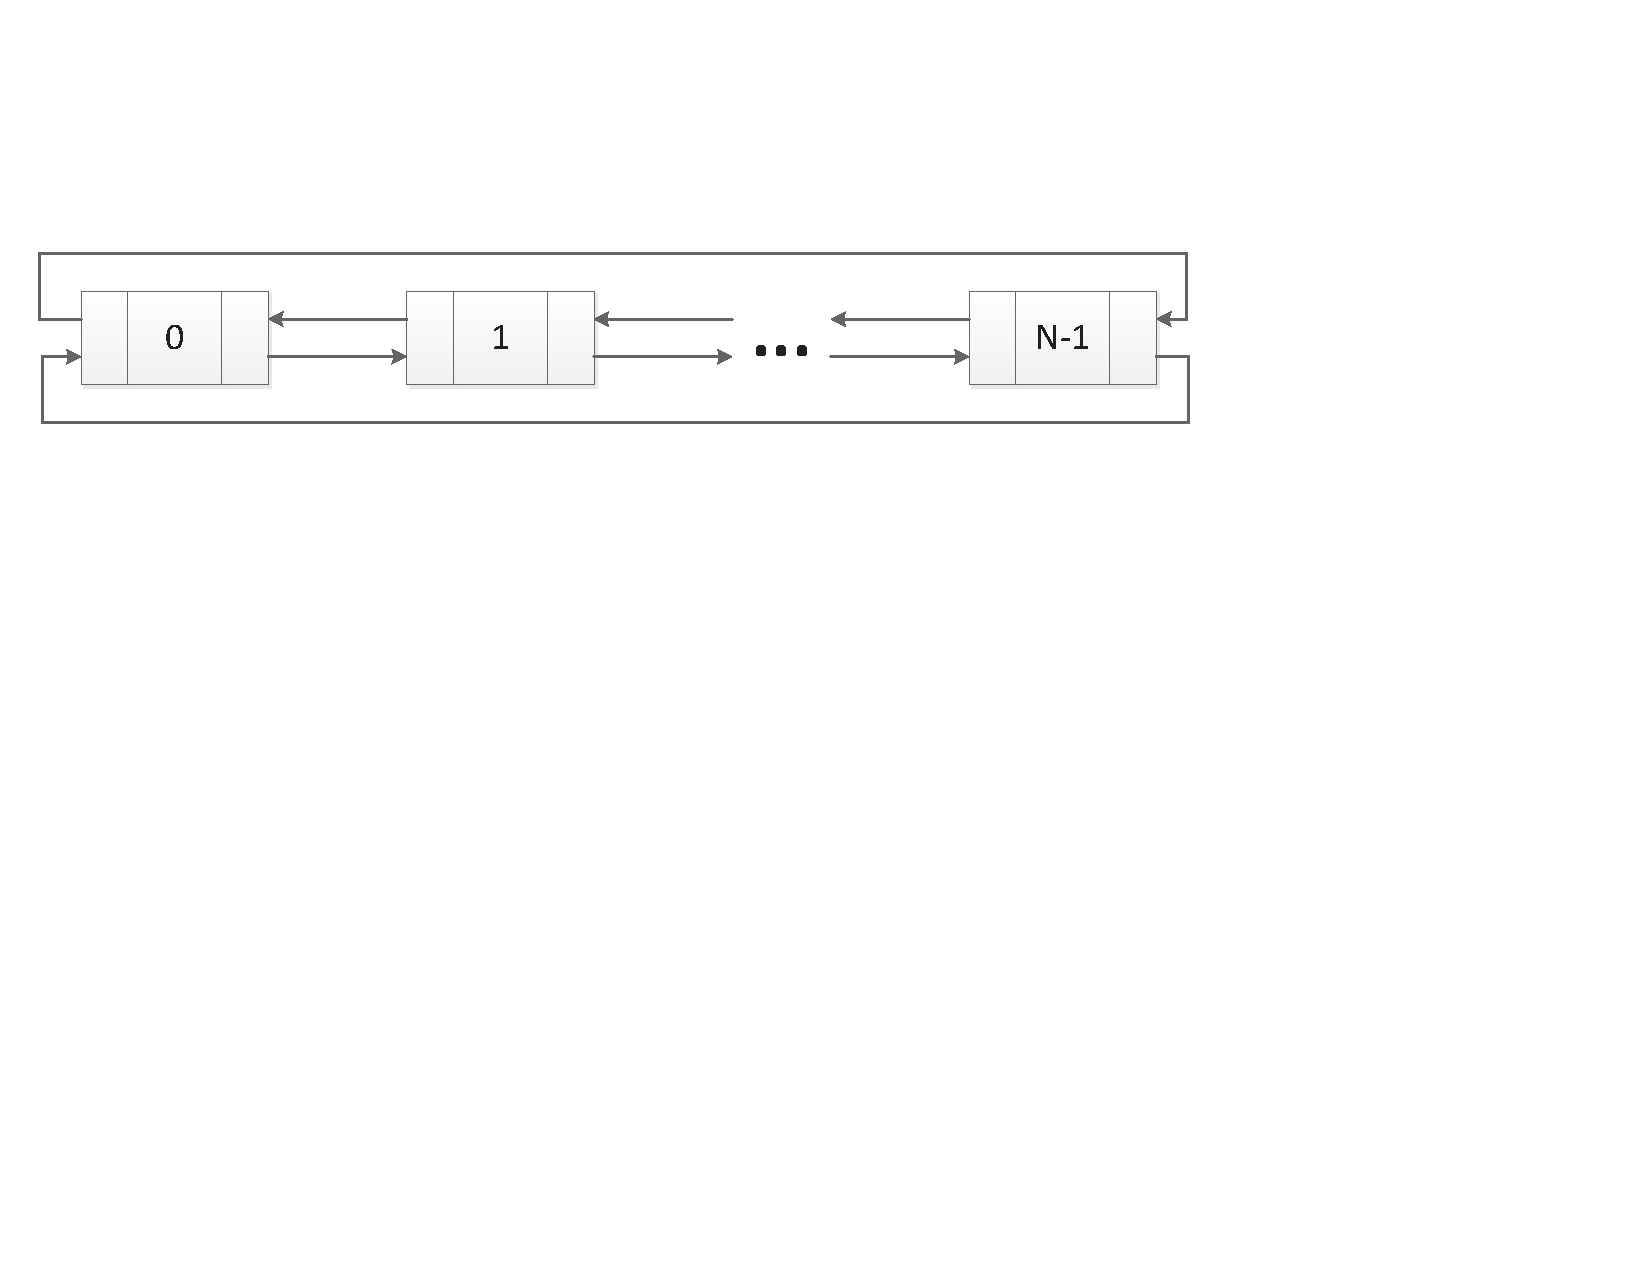
\includegraphics[width=0.6\textwidth, clip, keepaspectratio]{fig_init_boundary.eps}
\caption{N nodes circular doubly linked list structure}\label{fig:CircList}
\end{figure}

\vspace{1em}
{\setlength\parindent{0pt}
\textbf{Stack}\vspace{0.5em}}

Similar to the compression program, a user defined stack data structure is adopted by the decompression program. The fancy stack structure used in the decompression program requires an ability to delete an arbitrary element from the stack. A user defined stack structure named \lstinline!My_stack! is create, and the C++ standard list class is used as the base for \lstinline!My_stack! class, some additional functions are added.


\subsubsection{Decompression Preprocessing}
This procedure is used to preprocessing the compressed triangle mesh. It computes the number of triangles, number of external vertices and the offset for each S operation. Several variables and data structures need to be declared:

\begin{itemize}\itemsep=1.5pt
\item {\it t}, initialized to zero, tracks the number of triangles in the mesh.
\item {\it d}, initialized to zero, tracks the difference between the number of S and E operations. If $d < 0$, stop the preprocessing.
\item {\it e}, initialized to zero, final value of {\it e} represents the external vertices count.
\item {\it s}, initialized to zero, represents S operation count.
\item {\it ES stack}, initialized to empty. It saves (e, s) pair value.
\item {\it Offset table}, initialized to empty. It tracks how many vertices that must be skipped by each S operation.
\item {\it m}, initialized to zero, represents M operation count.
\item {\it m'}, initialized to zero, represents M' operation count.
\end{itemize}

The detailed description of those variables and data structures can also found in Table~\ref{tab:decompressInit}.
\begin{table}[h]
\normalsize
\centering
\caption{Decompression initialize variables}
  \begin{tabular}{ | c | p{0.75\textwidth} | }
    \hline
     Variables & Description \\
     \hline
     t & Triangle count, initialized to zero \\
     \hline
     d & Tracks the difference between the number of S and E operations. If d $< 0$, stop the preprocessing procedure. Initialized to zero.\\
     \hline
     e & External vertices count, initialized to zero \\
     \hline
     s & S operation count, initialized to zero \\
     \hline
     ES stack & Saves (e, s) pair, initialized to empty. \\
     \hline
     Offset table & Tracks how many vertices that must be skipped by each S operation, initialized to empty. \\
     \hline
     m & M operation count, initialized to zero \\
     \hline
     m' & M' operation count, initialized to zero \\
     \hline
    \hline
  \end{tabular}
  \label{tab:decompressInit}
\end{table}

The pseudo-code for all the variables update is denoted as:
\begin{algorithm}[H]
\caption{Decompression preprocessing}
\begin{algorithmic}[1]
\IF{C type triangle }
    \STATE{\lstinline!t += 1, e -= 1!}
\ELSIF{L type triangle}
    \STATE{\lstinline!t += 1, e += 1!}
\ELSIF{R type triangle}
    \STATE{\lstinline!t += 1, e += 1!}
\ELSIF{M type triangle}
    \STATE{\lstinline!t += 1, e -= (l + 1), m += 1!}
\ELSIF{M' type triangle}
    \STATE{\lstinline!t += 1, e -= 1, m' += 1!}
    \STATE{\{M' type pseudo-code is based on our best guess. Code is missing from the paper.\}}
\ELSIF{S type triangle}
    \STATE{\lstinline!t += 1, e -= 1, s += 1, d += 1, (e, s) = push!}
\ELSIF{E type triangle}
    \STATE{\lstinline!t += 1, e += 3, d -= 1, (e', s') = pop, O[s'] = e - e' - 2!}
    \IF{\lstinline!d < 0!}
        \STATE{stop the decompression preprocessing procedure}
    \ENDIF
\ENDIF
\end{algorithmic}
\end{algorithm}


From the description above, \lstinline!es_stack! is in standard integer pair type (\lstinline!std::pair<int, int> es_pair!). Each time when decompression program meets with an S operation, a pair of variables is pushed onto the stack. The top value pair is popped from the stack when the E operation is met. The current \lstinline!e! value and the \lstinline!s! value from the S operation are stored as a value pair, and then pushed to or popped from the stack.


\subsubsection{Triangle Mesh Decompression}
The triangle mesh decompression procedure is based on Edgebreaker's decompression algorithm and the parallelogram prediction scheme. It first creates the initial bounding loop based on the external vertices count, and then reconstructs the first two vertices position of the entire mesh (The reconstructed vertices are the two points with label \lstinline!0! and \lstinline!e! on the initial bounding loop). The triangle-vertex incident table (TV table) is generated based on the input op-code sequence. Each time when the decompression program generates a triangle facet, it will also reconstruct the position of the third vertex of the current triangle. The detailed TV table generation can be found in Section \ref{Sec:TVtable}. The circular doubly linked list update operation details can be found in Section \ref{sec:BEdgeUpdate}. The following pseudo-code is used for the triangle mesh decompression procedure.

\begin{algorithm}[H]
\caption{Triangle mesh decompression}
\begin{algorithmic}[1]
\STATE{Construct the initial bounding loop based on the external vertices count}
\STATE{Reconstruct two points with label \lstinline!0! and \lstinline!e! on the initial bounding loop}
\STATE{Define the stop condition for the do-while loop: \lstinline!bool e_case = false;!}
\STATE{Initialize the point for geometry reconstruction, \lstinline!updated_d = d !}
\REPEAT
    \STATE{Get the current triangle type from the op-code sequence vector}
    \STATE{Update the point for geometry reconstruction, \lstinline!d = updated_d!}
    \STATE{Update the processed triangle count: \lstinline!++triangle_cnt;!}
    \IF{C type triangle }
        \STATE{Update the TV table and the bounding loop}
        \STATE{Update the point for the next triangle \lstinline!updated_d!}
    \ELSIF{L type triangle}
        \STATE{Update the TV table and the bounding loop}
        \STATE{Update the point for the next triangle \lstinline!updated_d!}
    \ELSIF{R type triangle}
        \STATE{Update the TV table and the bounding loop}
        \STATE{Update the point for the next triangle \lstinline!updated_d!}
    \ELSIF{M type triangle}
        \STATE{Update the TV table and the bounding loop}
        \STATE{Update the point for the next triangle \lstinline!updated_d!}
        \STATE{Update the M type triangle count: \lstinline!m_cnt += 1!}
     \ELSIF{M' type triangle}
        \STATE{Update the TV table and the bounding loop}
        \STATE{Update the point for the next triangle \lstinline!updated_d!}
        \STATE{Update the M type triangle count: \lstinline!m'_cnt += 1!}
        \STATE{\{M' type pseudo-code is based on our best guess. Code is missing from the paper.\}}
    \ELSIF{S type triangle}
        \STATE{Update the TV table, geometry reconstruction for the third vertex of current triangle}
        \STATE{Push the left side sub mesh of the current S type triangle on the stack}
        \STATE{Update the point for the right side sub mesh \lstinline!d!}
        \STATE{Decompress the right side sub mesh of the current S type triangle}
        \STATE{Pop the stack, and decompress the left side sub mesh}
        \STATE{Update the point for the next triangle \lstinline!updated_d!}
    \ELSIF{E type triangle}
        \STATE{Update the TV table and the bounding loop}
        \STATE{No more triangle in current mesh, stop the compression, \lstinline!e_case = true;!}
    \ENDIF
    \IF{The third vertex of current triangle is \NOT predicted before}
        \STATE{Geometry reconstruction for the third vertex}
    \ENDIF
\UNTIL{\lstinline!\!e_case!}
\end{algorithmic}
\end{algorithm}


\subsection{Arithmetic Coding Binarization Scheme}
The integer prediction error between the actual position and predicted position is compressed by the binary arithmetic coding scheme. The binarization scheme we used in both compression and decompression programs are the n-bit unsigned integer with an adaptive nonuniform distribution. \cite{BinarizationScheme} The number of bits $n$ and the binarization parameter $f$ that employed in the binarization function $UI\{n, f\}$ will be determined during the implementation.


The context choose details for both the sign bit and the rest value bits are as follows. For the sign bit, the bypass mode is used. For all the value bits, the following two steps are employed to choose the context $c$ for each bit position $k$ from $n - 1$ down to $0$:

\begin{enumerate}
\item Code the $k$th bit $b_k$ using context $c$, where $c \in [0, 2^f + n - f - 1)$ and
\begin{align}
c = \begin{cases}
2^{f - 1} - 1 + \sum_{i \in [k + 1, f)} (2b_i - 1)2^{i-1}, & k \in [0, f - 1] \\
2^f - f + k - 1, & k \in [f, n - 1].
\end{cases}
\end{align}

\item If $b_k = 1$ and $k \geq f$, we code each of the remainning bits $\{b_i\}_{i \in [0, k)}$ in bypass mode.
\end{enumerate}




%%%%%%%%%%%%%%%%%%%%%%%%%%%%%%%%%%%%%%%%%%%%%%%%%%%%%%%%%%%%%%%%%%%%%%%%%%%
%           KEY CLASSES AND FUNCTIONS
%%%%%%%%%%%%%%%%%%%%%%%%%%%%%%%%%%%%%%%%%%%%%%%%%%%%%%%%%%%%%%%%%%%%%%%%%%%
\section{KEY CLASSES AND FUNCTIONS}
\subsection{Data Structure}
The \lstinline!Circ_list! class is a class which creates the circular doubly linked list data structure. The \lstinline!Circ_list! class is only used by the decompression program.\vspace{0.5em}

\lstinputlisting[basicstyle={\scriptsize\tt},numbers=left, stepnumber=1, numberstyle=\tiny, numbersep=10pt]{Circ_list.hpp}


\vspace{0.7em}
{\setlength\parindent{0pt}
\lstinline!My_findable_stack! class is a user defined stack class, it uses the C++ standard list class and the standard map class inside. This user defined stack can finds the internal element's position and deletes an arbitrary element from the stack. \lstinline!My_findable_stack! class is used in the compression program.

\lstinline!My_stack! class is a user defined stack class, the C++ standard list class is used inside the class. This user defined stack can deletes an arbitrary element from the stack. The \lstinline!My_stack! class is used in the decompression program.\vspace{0.5em}}

\lstinputlisting[basicstyle={\scriptsize\tt},numbers=left, stepnumber=1, numberstyle=\tiny, numbersep=10pt]{My_stack.hpp}


\vspace{0.7em}
{\setlength\parindent{0pt}
The arithmetic coding binarization scheme related class is stored in \lstinline!Context_selector.hpp! header file. This class is used for triangle mesh geometry encoding and decoding, and the \lstinline!Context_selector! class is included by both the compression and decompression programs.\vspace{0.5em}}

\lstinputlisting[basicstyle={\scriptsize\tt},numbers=left, stepnumber=1, numberstyle=\tiny, numbersep=10pt]{Context_selector.hpp}


\vspace{0.7em}
{\setlength\parindent{0pt}
The \lstinline!Mesh_handle! class is a class which stores each handle's information. This \lstinline!Mesh_handle! class is used by both the compression and decompression programs. The \lstinline!Mesh_handle! class is included in the \lstinline!Utility.hpp! header file. \vspace{0.5em}}

\vspace{0.7em}
{\setlength\parindent{0pt}
The \lstinline!Triangle_facet! class stores each triangle's three vertices label/index. This class is only used by the decompression program. The \lstinline!Triangle_facet! class is included in the \lstinline!Utility.hpp! header file.\vspace{0.5em}}

\vspace{0.7em}
{\setlength\parindent{0pt}
There are also some constants and functions that shared by both the compression and decompression programs. The definition or declaration of those shared information are all included in the \lstinline!Utility.hpp! header file. \vspace{0.5em}

\lstinputlisting[basicstyle={\scriptsize\tt},numbers=left, stepnumber=1, numberstyle=\tiny, numbersep=10pt]{Utility.hpp}


\subsection{Compression Program}
The main class contained in the compression program is \lstinline!Encoder!. All vertices contained in the triangle mesh have the type specified by the class \lstinline!My_Vertex!. The halfedges have the type specified by the class \lstinline!My_Halfedge!.\vspace{0.5em}

\lstinputlisting[basicstyle={\scriptsize\tt},numbers=left, stepnumber=1, numberstyle=\tiny, numbersep=10pt]{encoder.hpp}

\subsection{Decompression Program}
The main class used in the decompression program is the \lstinline!Decoder! class. For each triangle, the indices of composing vertices have the type specified by the class \lstinline!Label!. The circular doubly linked list structure used in the decompression program is \lstinline!Circ_list!.\vspace{0.5em}

\lstinputlisting[basicstyle={\scriptsize\tt},numbers=left, stepnumber=1, numberstyle=\tiny, numbersep=10pt]{decoder.hpp}



%%%%%%%%%%%%%%%%%%%%%%%%%%%%%%%%%%%%%%%%%%%%%%%%%%%%%%%%%%%%%%%%%%%%%%%%%%%
%           COMPRESSION ALGORITHM
%%%%%%%%%%%%%%%%%%%%%%%%%%%%%%%%%%%%%%%%%%%%%%%%%%%%%%%%%%%%%%%%%%%%%%%%%%%
\section{COMPRESSION ALGORITHM}
\subsection{Triangle Type Distinguish} \label{sec:triType}
Seven triangle topological relationships are adopted by the Edgebreaker algorithm. In order to give a brief introduce to those 7 types, the following notations are used. Let g represent the current half edge (i.e. the gate) of the triangle T, v be the vertex which not bounding the gate, and B represent the boundary of the mesh.

Seven types of topological relationship can be distinguished as follow: C (v is not on B), L (v immediately precedes g), R (v immediately follows g), E (v precedes and follows g), S (v is elsewhere on B), M (v is on hole's boundary), and M' (v is on handle's boundary). \cite{Edgebreaker} The detailed descriptions of those 7 triangle types are listed in Table~\ref{tab:triType}.

\begin{table}[h]
\normalsize
\centering
\caption{Triangle type distinguish}
  \begin{tabular}{ | c | p{0.85\textwidth} | }
    \hline
    Type & Description \\
    \hline
    C & If the third vertex v of the current triangle T hasn't be visited yet, which means it is not belongs to the bounding loop B \\
    \hline
    L & If the third vertex v of T belongs to B, and it's immediately precedes gate g \\
    \hline
    R & If the third vertex v of T belongs to B, and it is immediately follows gate g \\
    \hline
    E & If the third vertex v of T belongs to B, and it is immediately precedes and follows gate g \\
    \hline
    S & If the third vertex v of T belongs to B, and it is neither immediately precedes nor follows gate g \\
    \hline
    M & If the third vertex v of T belongs to hole's boundary \\
    \hline
    M' & If the third vertex v of T belongs to handle's boundary \\
    \hline
    \hline
  \end{tabular}
  \label{tab:triType}
\end{table}

In order to distinguish those 7 triangle types, a vertex mark has been introduced to indicate its status. Mark 0 represents the vertex hasn't be visited by the compression program yet, mark 1 represents vertex is previously visited, mark 2 represents vertex is located on the boundary of a hole, and mark 3 represents vertex is located on the boundary of a handle.

With the help of vertex mark, seven types of triangles can be easily distinguished. If third vertex's mark equals to zero, current triangle is in C type. If vertex's mark is 2, triangle is in M type. If vertex's mark is 3, triangle is in M' type. Otherwise, the current triangle is in L, E, R, or S type. The distinguish between those four types can be achieved by the relationship between the vertex v and the gate g. The pseudo code for the triangle type distinguish is denoted as (The g.v.m notation is used to represent the vertex's mark):

\begin{algorithm}[H]
\caption{Triangle type distinguish}
\begin{algorithmic}[1]
\IF{\lstinline!g.v.m == 0!}
    \STATE{C type triangle}
\ELSIF{\lstinline!g.v.m == 2!}
    \STATE{M type triangle}
\ELSIF{\lstinline!g.v.m == 3!}
    \STATE{M' type triangle}
\ELSE
    \IF{\lstinline!g -> next() -> is_border_edge()!}
        \IF{\lstinline!g -> prev() -> is_border_edge()!}
            \STATE{E type triangle}
        \ELSE
            \STATE{R type triangle}
        \ENDIF
    \ELSE
        \IF{\lstinline!g -> prev() -> is_border_edge()!}
            \STATE{L type triangle}
        \ELSE
            \STATE{S type triangle}
        \ENDIF
    \ENDIF
\ENDIF
\end{algorithmic}
\end{algorithm}


\subsection{Gate Update} \label{sec:gateUpdate}
Based on the Edgebreaker's compression algorithm, for C, L and M type triangle, the active gate is updated to the opposite half edge of the current gate's next half edge around the facet, i.e., \lstinline!g -> next() -> opposite()!. For R type triangle, the gate is updated to the opposite half edge of the current gate's previous half edge around the facet, i.e., \lstinline!g -> prev() -> opposite()!.

For S type triangle, it splits the current mesh into two pieces, the algorithm compresses the right side sub-mesh first and then moves to the left side sub-mesh. So the gate of the S type triangle updates to \lstinline!g -> next() -> opposite()! first, and then moves to \lstinline!g -> prev() -> opposite()!. For E type triangle, it's the last triangle of the current stream, so it pops the stack. For M' type triangle, since it's pseudo-code is missing from the paper, our best guess is the active gate for M' type is update to \lstinline!g -> next() -> opposite()!. The gate update pseudo-code for each type of triangle's is listed below:

\begin{algorithm}[H]
\caption{Gate update}
\begin{algorithmic}[1]
\IF{C \OR L \OR M type triangle }
    \STATE{active gate updates to: \lstinline!g -> next() -> opposite()!}
\ELSIF{M' type triangle }
    \STATE{active gate updates to: \lstinline!g -> next() -> opposite()!}
    \STATE{\{M' type pseudo-code is based on our best guess. Code is missing from the paper.\}}
\ELSIF{R type triangle}
    \STATE{active gate updates to: \lstinline!g -> prev() -> opposite()!}
\ELSIF{S type triangle}
    \STATE{active gate updates to: \lstinline!g -> next() -> opposite()!, compress the right side sub-mesh}
    \STATE{active gate updates to: \lstinline!g -> prev() -> opposite()!, compress the left side sub-mesh}
\ELSIF{E type triangle}
    \STATE{last triangle in current stream, pop the stack}
\ENDIF
\end{algorithmic}
\end{algorithm}


\subsection{Point Update} \label{sec:vetexUpdate}
The parallelogram prediction scheme predict as the fourth vertex of a parallelogram from the other three vertices. Two of the three known points are come from the start and end point of the current active gate. The third known point is from the last processed triangle. Under this circumstance, we need to update the third known point for the next triangle.

For the C, L and M type of triangle, the point is update to start point of the current gate. For the R type, the point is update to gate's end point. For S type triangle, the third known point updates to the gate's start point first (for the right side sub-mesh), then updates to the gate's end point for the left side sub-mesh. For M' type of triangle, since the point update details is missing from paper, we think the point is update to start point of the current gate. For E type triangle, it's the last triangle of the current stream, so there is no point update performance. The pseudo-code for point update is as follows:


\begin{algorithm}[H]
\caption{Point update}
\begin{algorithmic}[1]
\IF{C \OR L \OR M type triangle }
    \STATE{Point updates to: \lstinline!gate -> opposite() -> vertex() -> point();!}
\ELSIF{M' type triangle }
    \STATE{Point updates to: \lstinline!gate -> opposite() -> vertex() -> point();!}
    \STATE{\{M' type pseudo-code is based on our best guess. Code is missing from the paper.\}}
\ELSIF{R type triangle}
    \STATE{Point updates to: \lstinline!gate -> vertex() -> point();!}
\ELSIF{S type triangle}
    \STATE{Point updates to: \lstinline!gate -> opposite() -> vertex() -> point();! for the right side sub-mesh}
    \STATE{Point updates to: \lstinline!gate -> vertex() -> point();! for the left side sub-mesh}
\ELSIF{E type triangle}
    \STATE{Last triangle in current stream, no point update performance}
\ENDIF
\end{algorithmic}
\end{algorithm}



%%%%%%%%%%%%%%%%%%%%%%%%%%%%%%%%%%%%%%%%%%%%%%%%%%%%%%%%%%%%%%%%%%%%%%%%%%%
%           DECOMPRESSION ALGORITHM
%%%%%%%%%%%%%%%%%%%%%%%%%%%%%%%%%%%%%%%%%%%%%%%%%%%%%%%%%%%%%%%%%%%%%%%%%%%
\section{DECOMPRESSION ALGORITHM}
\subsection{Circular Doubly Linked List Structure Initialization}
To initialize the circular doubly linked list structure, the decompression program creates a circular doubly linked list structure with e number of nodes. The first node is assigned with label 0, and the labels of the rest e - 1 nodes are assigned by successive increments 1 from the previous node. The recursive triangle-vertices incidence table generation procedure is starts from the node with label zero.


\subsection{Circular Doubly Linked List Structure Update} \label{sec:BEdgeUpdate}
During the triangle-vertices incident table generation procedure, each time when the decompression program reads an op-code, it updates the elements in the circular doubly linked list structure. For C type op-code, one node with label $e + 1$ is introduced between G.P.e and G.e node. For L type triangle, the G.P.e node is deleted from the structure; for R type triangle, the G.e node is deleted; for E type op-code, three nodes: G.e, G.P.e and G.N.e are deleted. For S type op-code, the decompression program splits the current circular doubly linked list structure into two parts, the first sub circular doubly linked list structure connects the D.e node with G.e node directly; for the second sub structure, it contains nodes from G.P.e to D.e from the origin circular doubly linked list structure.

For M' type op-code, the decompression program create a new edge A. Due to the missing details in the paper, I guess the index of this new edge A is \lstinline!A.e = D.e!. This new node with label A.e is added between the node G.P.e and D.e.

For M type op-code, an extra $l + 1$ nodes are introduced to the bounding loop, where {\it l} represents the length of current hole. Those $l + 1$ nodes are inserted between the node G.P.e and G.e. The label for the last node is $e + 1$. The labels of the first {\it l} nodes are assigned by successive increments of {\it e}. A short diagram in Fig.~\ref{fig:typeM_boundary} shows the bounding loop structure after M op-code finish its updates.

\begin{figure}[h]
\centering
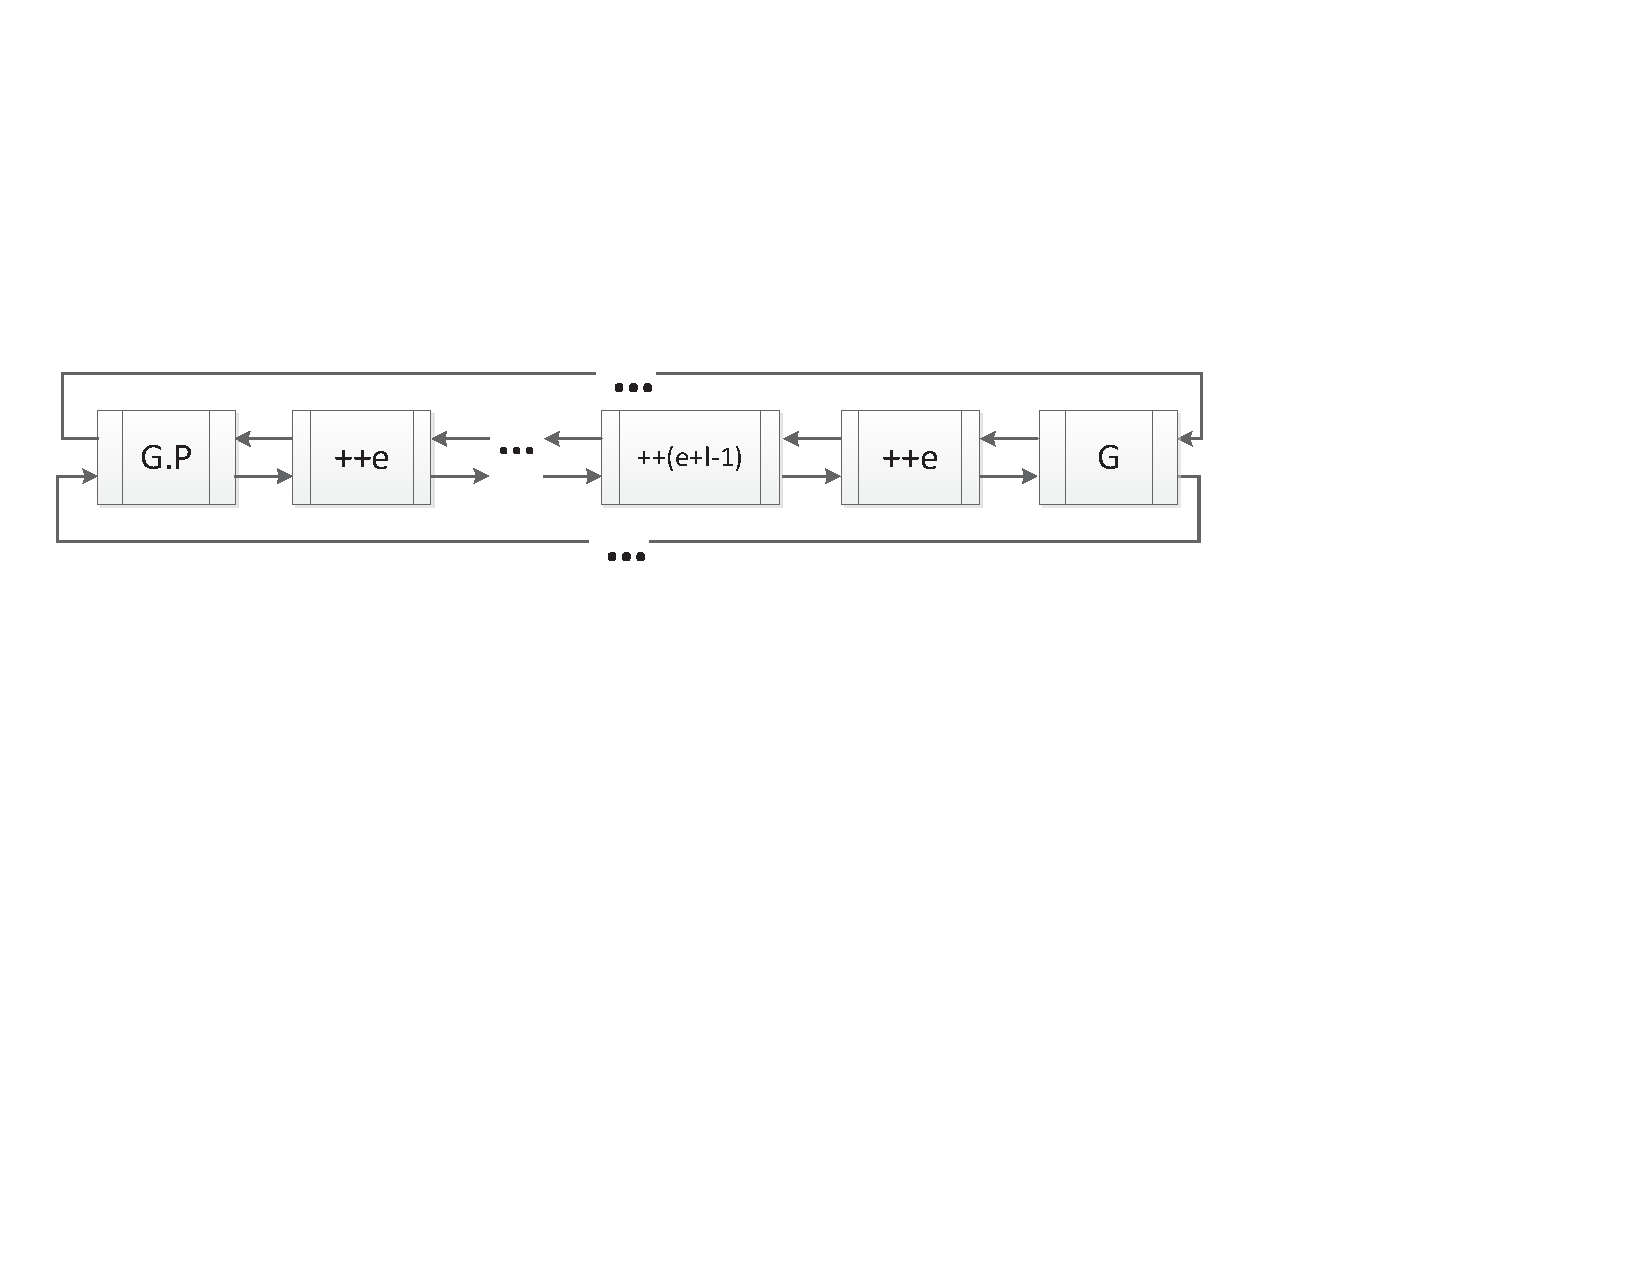
\includegraphics[width=0.7\textwidth, clip, keepaspectratio]{fig_typeM_boundary.eps}
\caption{Bounding loop structure after M type op-code}\label{fig:typeM_boundary}
\end{figure}

Based on the description above, the pseudo-code of circular doubly linked list structure update can be written as:

\begin{algorithm}[H]
\caption{circular doubly linked list structure update}
\begin{algorithmic}[1]
\IF{C type triangle}
    \STATE{Insert \lstinline!++e! node between \lstinline!G.P.e! and \lstinline!G.e!}
\ELSIF{L type triangle}
    \STATE{Delete node \lstinline!G.P.e!, connect \lstinline!G.P.P.e! and \lstinline!G.e! directly}
\ELSIF{R type triangle}
    \STATE{Delete node \lstinline!G.e!, connect \lstinline!G.P.e! and \lstinline!G.N.e! directly}
\ELSIF{E type triangle}
    \STATE{Delete three nodes: \lstinline!G.e, G.P.e! and \lstinline!G.N.e!}
\ELSIF{S type triangle}
    \STATE{\lstinline!D.e = G.N.e;!}
    \FOR{$i = 0$ to O[++s]}
        \STATE{\lstinline!D.e = D.N.e!}
    \ENDFOR
    \STATE{Connect \lstinline!D.e! and \lstinline!G.e! directly, generate TV table for the right side sub BEdge structure}
    \STATE{Connect \lstinline!G.P.e! and \lstinline!D.e! directly, generate TV table for the left side sub BEdge structure}
\ELSIF{M type triangle}
    \STATE{Insert (l + 1) nodes between G.P.e and G.e, with first l nodes are assigned by successive increments of e, and the the last one node assigned with label e + 1}
\ELSIF{M' type triangle}
    \STATE{Create node \lstinline!A.e!, insert this \lstinline!A.e! node between \lstinline!G.P.e! and \lstinline!D.e!}
    \STATE{\{M' type pseudo-code is based on our best guess, part of the code is missing in the paper.\}}
\ENDIF
\end{algorithmic}
\end{algorithm}


\subsection{Triangle-vertex Incidence Table Generation} \label{Sec:TVtable}
According to the Edgebreaker's decompression algorithm, the first two vertices label/index of each triangle are always the current vertex's index: G.e, and the previous vertex's index: G.P.e, in the circular doubly linked list structure. The only difference for each type of triangle is the third vertex's index.

For C and M type triangle, it introduces new vertex to the current circular doubly linked list structure, so the third vertex's index is the increment of the current \lstinline!e! count (i.e., \lstinline!++e!). For R and E type of triangle, the third vertex's index is next vertex's index of G (i.e., \lstinline!G.N.e!). For L type triangle, the third vertex's label is previous vertex's index of G.P (i.e., \lstinline!G.P.P.e!).

For S type triangle, it first generates the vertex's index D.e, which is the next vertex's index of G (i.e., \lstinline!D.e = G.N.e!), and then repeats \lstinline!D.e = D.N.e! for O[++s] times, the vertex index of final D (i.e., \lstinline!D.e!) is used as the third vertex's label of S triangle.

For M' type triangle, it first generates the vertex's index D.e, which is the next vertex's index of G (i.e., \lstinline!D.e = G.N.e!), and then repeats \lstinline!D.e = D.N.e! for o times (o represents the offset value for current M' triangle), the vertex index of final D (i.e., \lstinline!D.e!) is used as the third vertex's label of M' triangle. The vertices indices for each type of triangle can be represented as:

\begin{algorithm}[H]
\caption{TV table generation}
\begin{algorithmic}[1]
\IF{C type triangle}
    \STATE{Three indices: \lstinline!(G.P.e, G.e, ++e)!}
\ELSIF{L type triangle}
    \STATE{Three indices: \lstinline!(G.P.e, G.e, G.P.P.e)!}
\ELSIF{R type triangle}
    \STATE{Three indices: \lstinline!(G.P.e, G.e, G.N.e)!}
\ELSIF{E type triangle}
    \STATE{Three indices: \lstinline!(G.P.e, G.e, G.N.e)!}
\ELSIF{S type triangle}
    \STATE{\lstinline!D.e = G.N.e;!}
    \FOR{$i = 0$ to O[++s]}
        \STATE{\lstinline!D.e = D.N.e!}
    \ENDFOR
    \STATE{Three indices: \lstinline!(G.P.e, G.e, D.e)!}
\ELSIF{M type triangle}
    \STATE{Three indices: \lstinline!(G.P.e, G.e, ++e)!}
\ELSIF{M' type triangle}
    \STATE{\lstinline!D.e = G.N.e;!}
    \FOR{$i = 0$ to o}
        \STATE{\lstinline!D.e = D.N.e!}
    \ENDFOR
    \STATE{Three indices: \lstinline!(G.P.e, G.e, D.e)!}
\ENDIF
\end{algorithmic}
\end{algorithm}



%%%%%%%%%%%%%%%%%%%%%%%%%%%%%%%%%%%%%%%%%%%%%%%%%%%%%%%%%%%%%%%%%%%%%%%%%%%
%          APPENDIX
%%%%%%%%%%%%%%%%%%%%%%%%%%%%%%%%%%%%%%%%%%%%%%%%%%%%%%%%%%%%%%%%%%%%%%%%%%%
\begin{appendices}
\section{Missing Details from the M' Type of Triangle}
In Section7.2 Handles of the Edgebreaker's paper, the author gives us very brief description about how to handle the general meshes with one or more handles. Unfortunately, some very important details are missing from the paper.


\subsection{Missing Details from Compression Algorithm}
The compression pseudo-code for M' type of triangle is completely missing from the paper. Based on author's description, we can understand some parts of the compression algorithm. There still some problems left, the items list below are the unsolved issues for the M' type:

\begin{itemize}
\item When meet with M' type triangle during the compression procedure, should the compression algorithm updates the vertices and halfedges mark from 3 to 1? From Section4 Compressing Simple Meshes of the original Edgebreaker's paper, vertex with mark 1 means this vertex is visited before, and halfedge with mark 1 means this halfedge is included in the current bounding loop. Since both the vertices and the halfedges are met by the M' type triangle, I think the compression algorithm should updates the vertices and halfedges mark.
\item The M' compression algorithm calculates the position p. Does this position p represent the distance between the associated gate and the beginning element in the stack?
\item For the offset o between the associated gate and the reached point, does this offset value in the integer type? The associated gate is an halfedge handle and the reached point is a mesh vertex. The gate and the reached point are not in the same type. Therefore, how could we calculate the offset between a halfedge handle and an vertex?
\end{itemize}


\subsection{Missing Details from Decompression Algorithm}
Although the Edgebreaker's paper contains the decompression pseudo-code for the M' type triangle, the explanation of M' type decompression is not clear enough. The unclear points are list as follows:

\begin{itemize}
\item Since there is no description about the M' type decompression preprocessing operation, we don't know how many vertices are subtract from the external vertices count. My best conjecture about the value that needs to subtract is relate to the offset value o. Besides the external vertices count adjustment, we don't know whether the M' type op-code requires other operation in the decompression preprocessing phase.
\item The first step for M' type decompression is to fetches and removes entry p from the stack. Does this imply the decompression algorithm requires a fancy stack structure that allows its user to remove the internal element?
\item The decompression pseudo-code mentions create new edge (edge A) in the current bounding loop. For this new edge A, what's the value of A.e? Does the value of A.e relate to the value of D.e?
\end{itemize}


\section{Error Correction in Edgebreaker's Paper}
\subsection{Pseudo-code for Case M Compression}
The sequence of fix links and traversal edges on the hole in M type compression is reversed. We should traversal the edges on the hole first, then fix the links. The purpose of traversal the edges of the hole is to update the vertices and halfedges mark, calculate the hole's length, and also append all hole's vertices to the point list. The purpose of fix links is to update the successor and predecessor relationships for all the halfedges on the current boundary loop. (At this point, the hole is part of the boundary loop.)

If we fix links first, then the current hole is become part of the bounding loop. Then all the update vertices and halfedges work we done are not on the hole, but on the original bounding loop (the loop before we processing the current M type triangle).

Also, the pseudo-code for traversal the edges on the hole has some problems. Rossignac's code can only traversal \lstinline!(hole_length - 1)! edges on the boundary. The hole's beginning edge, edge \lstinline!b! is not visited by the code. The correct pseudo-code for M type compression is as follows:
\begin{algorithm}[H]
\caption{Pseudo-code for M type compression}
\begin{algorithmic}[1]
\STATE{\lstinline!H=H|M;!} \COMMENT{append M to history}
\STATE{\lstinline!g.m=0; g.p.o.m=1; g.n.o.m=1;!}  \COMMENT{update marks}
\STATE{\lstinline!b=g.n;!}  \COMMENT{initial candidate for b}
\WHILE{\lstinline!b.m\!=2!}
    \STATE{\lstinline!b=b.o.p;!} \COMMENT{turn around v}
\ENDWHILE

\STATE{\lstinline!l=0;!} \COMMENT{initial hole length count}
\REPEAT
    \STATE{\lstinline!b.m=1; b.e.m=1;!} \COMMENT{mark hole}
    \STATE{\lstinline!l++;!} \COMMENT{counts length of hole}
    \STATE{\lstinline!P=P|b.e;!} \COMMENT{append new vertex reference to P}
    \STATE{\lstinline!b=b.N!} \COMMENT{move to next edge around hole}
\UNTIL{\lstinline!\!b.e\!=g.v;!}
\STATE{\lstinline!L=L|l;!} \COMMENT{appends the length of hole to L}

\STATE{\lstinline!g.P.N=g.p.o; g.p.o.P=g.P;!} \COMMENT{fix red link 1 in B}
\STATE{\lstinline!g.p.o.N=b.N; b.N.P=g.p.o;!} \COMMENT{fix red link 2 in B}
\STATE{\lstinline!b.N=g.n.o; g.n.o.P=b;!} \COMMENT{fix red link 3 in B}
\STATE{\lstinline!g.n.o.N=g.N; g.N.P=g.n.o;!} \COMMENT{fix red link 4 in B}
\STATE{\lstinline!g=g.n.o; StackTop=g!} \COMMENT{move g}
\end{algorithmic}
\end{algorithm}


\subsection{Pseudo-code for the Decompression Preprocessing}
The subtraction operation sign is missing from several places in the decompression preprocessing pseudo-code. Based on the decompression algorithm, for S and C type of triangle, both of the op-codes subtract one vertex from the external vertices count \lstinline!e!. For E op-code, it decrease the \lstinline!d! count by one.

The decompression preprocessing operation for M op-code is only described in the algorithm, the author did not list the M type decompression preprocessing pseudo-code with other types. For M type of triangle, it decrease \lstinline!(l + 1)! vertices from the external vertices count \lstinline!e!. The correct pseudo-code for each type of triangle is listed below:

\begin{algorithm}[H]
\caption{Pseudo-code for the decompression preprocessing}
\begin{algorithmic}[1]
\STATE{Case S: \lstinline!e -= 1; s += 1; push(e, s); d += 1;!}
\STATE{Case E: \lstinline!e += 3; (e', s') = pop; O[s'] = e - e' - 2; d -= 1;! If \lstinline!d < 0;! then stop.}
\STATE{Case C: \lstinline!e -= 1; c += 1;!}
\STATE{Case R: \lstinline!e += 1;!}
\STATE{Case L: \lstinline!e += 1;!}
\STATE{Case M: \lstinline!e -= (l + 1);!}
\end{algorithmic}
\end{algorithm}


\subsection{Figure. 12 for the Case M}
For M type of triangle, there is no halfedge that needs to be pushed onto the stack. In the right side sub-figure of Figure.~12 in the Edgebreaker's paper, the halfedge currently has the ``Push'' notation should be a normal halfedge without any notation.

\end{appendices}



%%%%%%%%%%%%%%%%%%%%%%%%%%%%%%%%%%%%%%%%%%%%%%%%%%%%%%%%%%%%%%%%%%%%%%%%%%%
%          REFERENCE
%%%%%%%%%%%%%%%%%%%%%%%%%%%%%%%%%%%%%%%%%%%%%%%%%%%%%%%%%%%%%%%%%%%%%%%%%%%
\begin{thebibliography}{99}
\bibitem{Edgebreaker}
J. Rossignac,  \emph{Edgebreaker:  Connectivity  compression  for triangle  meshes}, IEEE Transactions on Visualization and Computer Graphics, Vol. 5, No. 1, January - March 1999.

\bibitem{Parallel}
C. Touma and C. Gotsman, \emph{Triangle Mesh Compression}, Proceedings Graphics Interface 98, pp. 26-34, 1998

\bibitem{3.67v}
D. King and J. Rossignac, \emph{Guaranteed 3.67v bit encoding of planar triangle graphs}, In Proc. 11th Canadian Conf. On Computational Geometry, Vancouvert, August 1999

\bibitem{predictScheme}
http://www.cc.gatech.edu/~jarek/edgebreaker/eb/PredictionScheme.htm

\bibitem{BinarizationScheme}
M. D. Adams, \emph{An efficient progressive coding method for arbitrarily-sampled image data}, IEEE Signal Processing Letters, vol. 15, pp. 629-632, 2008.

\end{thebibliography}

\end{document}
